% chap4.tex (Definitions and Theorem)

\chapter{Storage Optimization Framework for Provenance Data Storage in IoT devices} \label{MostNarrowEasy}

In this chapter, we define our model and algorithms for storage optimization of provenance data in IoT. We focus on our proposed data pruning technique. We evaluate our hypothesis using the proof of concept ideology.

%\section{Definitions}
%
%\begin{definition}
%{\rm We say that the number $\tilde x$ represents a number $x$ with
%{\em absolute accuracy\/} $\Delta>0$ if $|x-\tilde x|\leq\Delta$.}
%\end{definition}
%
%\begin{definition}
%{\rm By {\em absolute half-width\/} of the interval ${\bf x}=[x^-,x^+]$, we
%mean the smallest number $\Delta>0$ for which every number in ${\bf x}$ is
%represented with an absolute accuracy~$\Delta$ by $\tilde x=\displaystyle{
%\frac{x^-+x^+}{2}}$.\\[0.5pc]
%{\bf Proposition} It can be seen that the absolute half-width of ${\bf x}$ is
%$$
%  \max_{x\in [x^-,x^+]} |x-\tilde x| = \frac{x^+-x^-}{2}.
%$$}
%\end{definition}


\section{A policy-based approach to efficient provenance storage}
\par Provenance generates more data than the data in which provenance is being collected. Due to the large influx of real-time data generated from sensor and actuators in IoT, we envision large amounts of provenance data will generated from our provenance collection framework. The resource constraints on the sensor/actuator and the device layer of the IoT architecture makes it even more challenging. There is a need to create an efficient storage framework for storing provenance data. To address this issue, we define a policy driven framework that provides a policy scheme for the enforcement of provenance storage. Policy approach allows the flexibility of provenance selection. A policy approach makes selecting what provenance is considered important to a specific IoT architecture thereby eliminating irrelevant provenance information. Since various organizations have varied provenance requirement(s), making provenance static might not be suitable across all IoT architecture. The approach of using policy for enforcement is slightly different from the typical access control approach. In other words, Policy is used for the resource enforcement of provenance data collected. This enables efficient pruning of provenance data in which all irrelevant data discarded. The policy framework consists of a policy document. This document contains information on provenance data that is considered relevant to the IoT architecture. A policy framework is used to address resource constraints encountered when storing large amounts of provenance data on low memory devices. Policy document is created by a user who serves as an administrator.  An administrator is a user which has the right to add, delete or modify a policy document. For implementation, there are several policy models that can be utilized to integrate a policy model with the IoT framework. 

\par Our policy architecture is modeled using the Common Open Policy Service(COPS) Standard \cite{rfc2748}. COPS consists of components for policy generation, evaluation and enforcement. The Policy Enforcement Point (PEP) enforces decisions received from the Policy Decision Point (PDP). The PDP evaluates policies and generates decision based on the evaluation. The model is extended to include a secondary decision point(SDP). This allows for distributed policy evaluation, freeing up the PDP from communication bottlenecks caused by large amounts of request received by a single PDP.  The figure below illustrates the system architecture of our proposed framework. Various layers of the IoT architecture contains different components of the decision and enforcement model. The Sensor/actuator layer of the IoT architecture is omitted. This is due tot he fact that this layer has the largest amount of memory restraints. Additionally, sensors and actuators are contained in the device layer and and as such does not require that data be pruned at this layer. 

\begin{figure}[h!]
\begin{center}
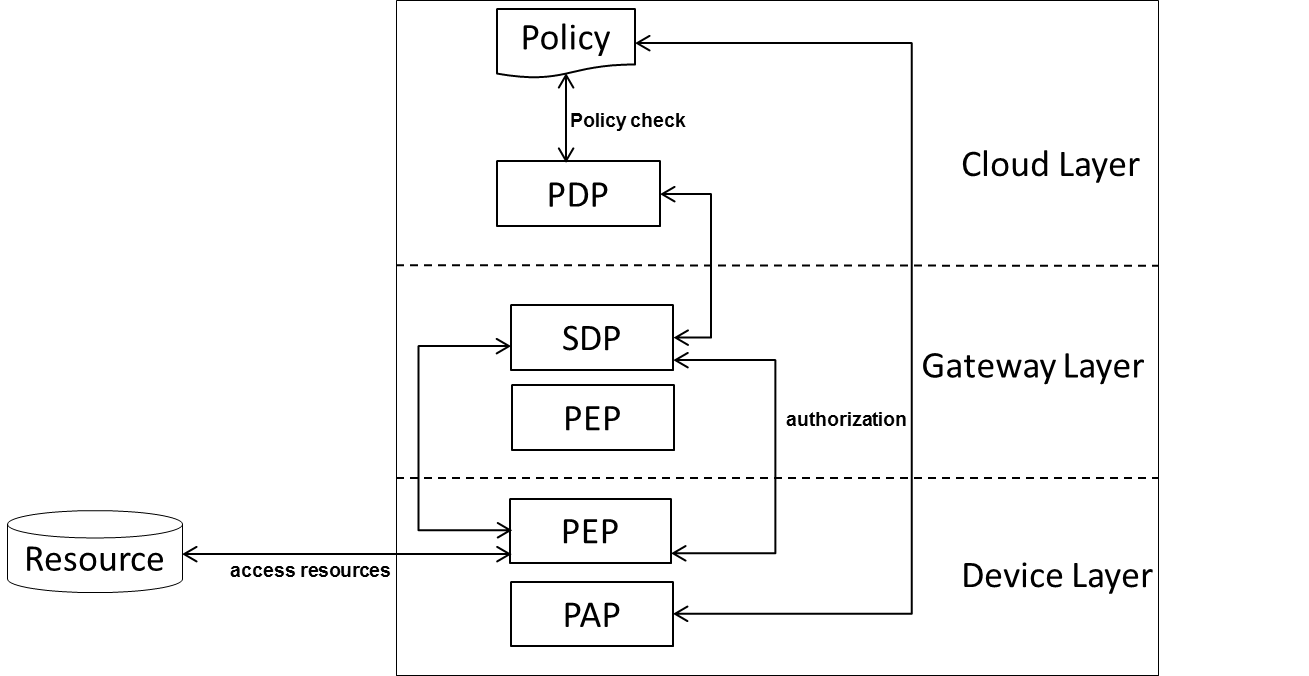
\includegraphics[height=3.5in]{policy_architecture.png}
\caption{Policy based system architecture which allows for effective data storage of provenance data}
\end{center}
\end{figure}


Policy document is generated at the device layer and evaluated at the gateway and cloud layer. The PEP which is involved with generating requests is located in the device and gateway layer. SDP is located in the gateway layer. This allows for policy evaluation without inuring additional network overhead of communicating with the PDP located in the cloud layer. To implement our policy based framework, We propose to use the eXtensible Markup Language(XACML) policy model \cite{xacml} to generate and enforce provenance policy for our IoT framework. We extend XACML to include the SDP component.

\subsection{eXtensible Access Control Markup Language}
 XACML is an access control policy language that allows the creation and enforcement of policies written in XML. It is a standard specification developed by the Organization of Advancement of Structured Information Standards(OASIS). Since it is written in XML, this framework allows for extensible and flexible policy documents. XACML consists of three major components which are involved in policy generation, evaluation and enforcement. The components of XACML are described below: 
 
 
 \begin{itemize}
 
 \item Policy Administration Point (PAP): This component of XACML
is involved with the generation of policy documents. A Policy document is created by specifications and requirements set aside by an administrator.

 \item Policy Decision Point (PDP): The Policy Decision Point evaluates policies by the request context generated by a user. Based on the request, It generates a response(accept,deny or intermediate) This response is communicated with the Policy Enforcement Point which enforces the response sent by the PDP.


\item Policy Enforcement Point (PEP):  The Policy Enforcement Point generates request context which is sent to the PDP for evaluation. It is also involved with the responsibility of enforcing request based on decision received by the PDP.

 \end{itemize}
 
 
 
 \begin{figure}[h!]
\begin{center}
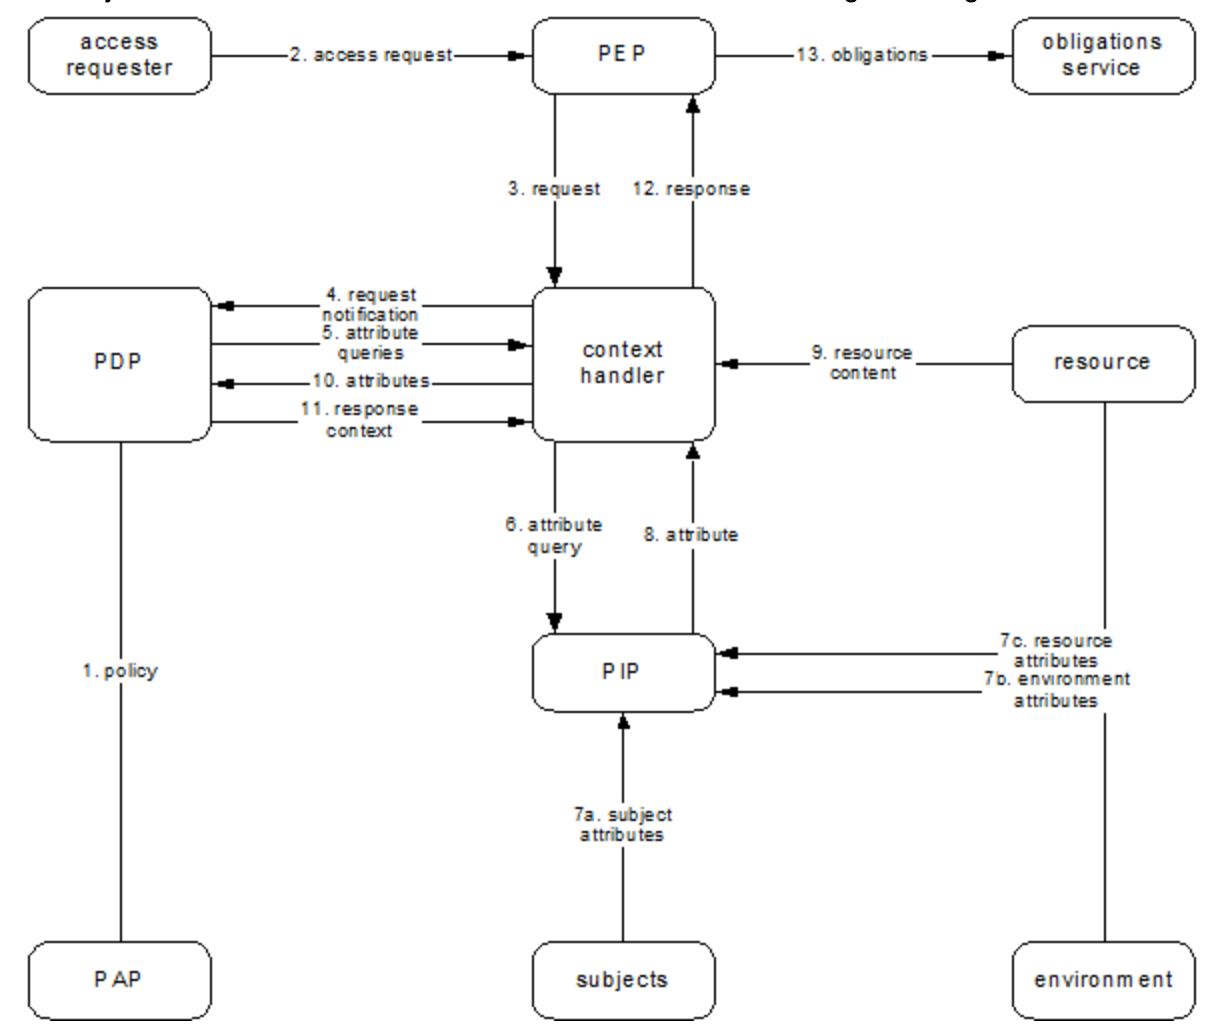
\includegraphics[height=3.5in]{xacml.png}
\caption{Xacml Data-flow diagram}
\end{center}
\end{figure}

\par Using the use case of the smart home depicted in chapter 2, a policy framework could be implemented and incorporated into the IoT which allows a device administrators to specify what kinds of provenance data to collect. The policy acts an enforcement point providing an efficient storage mechanism in a resource constrained environment. The contents of the implementation details for the policy framework which specifies the policy grammar and the policy architecture across the IoT stack are left as future work.


\section{Provenance-model Information Flow}

This section details how various components of IoT provenance collection system are combined. Figure \ref{flow_chart} depicts a flowchart which illustrates how provenance is generated and how policy is used to enforce access on provenance data. Input documents are represented in green while processes are represented by the blue. Document of various components contained in the flowchart are needed as input parameters to the processes that makes up the architecture. Policy document is generated by an administrator who decides what kinds of provenance data to collect. The administrator can be a device owner who has access and authority to the device. A yaml configuration file is passed as an input to the the tracer component. The yaml configuration is a essential portion of the tracer system.  It is used to generate application CTF trace output. It contains instructions of what trace data to collect. The policy framework takes a modular approach. Policy component can be added at various layers of the IoT architecture. The policy engine is involved with the authorization and enforcement of policies generated. This portion generates a decision based on the policy evaluation. The response from the policy allows provenance effectively pruned. Provenance data stored as CTF trace which is mapped to PROV-JSON format. The PROV-JSON serialization is used as input to our IDS system. Figure \ref{flow_chart} below illustrates the relationship between various component in the provenance aware IoT framework.

\begin{figure}[h]
\begin{center}

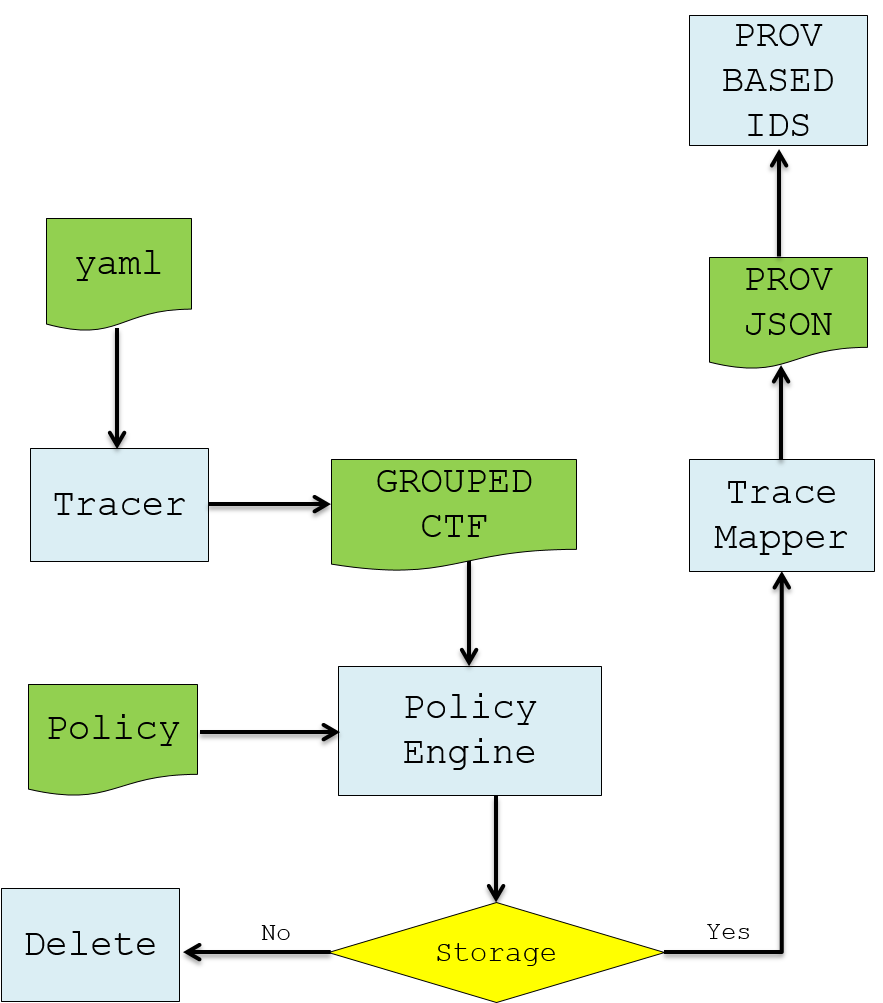
\includegraphics[width =4.5in]{flowchart.PNG}    
\end{center}
\caption{Architectural Flowchart }
\label{flow_chart}
\end{figure}




%\section{Proposed Research Experiment Evaluation}
%
%We plan to evaluate the effectiveness of our approach for the provenance collection framework and our framework for efficient provenance storage by running an intusion detection system for IoT device. An IDS is used to detect malicious attacks based on a certain policy or thresehold set by an administrator. There are two types of  IDS: Rule-based apprach, or anomaly based apporach. The rule based approach allows for intrusion monitoring based on rules specified by an adminstrator. On the other hand, anomaly based IDS which monitors intrusion based on patterns that falls out of the normal system function. Most anomaly\-based approach deals with machine learning to classify normal or anomalous behaviour.  

%\begin{definition}
%{\rm By {\em absolute width\/} $W$ of an interval ${\bf x}=[x^-,x^+]$, we mean
%twice the absolute half-width of ${\bf x}$, i.e.,
%$$
%  W([x^-,x^+])=x^+-x^-.
%$$}
%\end{definition}
%
%\begin{definition}
%{\rm We say that an interval ${\bf x}$ is {\em $\Delta$-narrow in the sense
%of absolute accuracy\/} if $W({\bf x})\leq\Delta$.}
%\end{definition}
%
%\begin{definition}
%{\rm Let $\varepsilon>0$ be a real number, let $D\subseteq R^N$ be a closed
%and bounded set of positive $N$-dimension volume $V(D)>0$, and let
%$P(x)$ be a property that is true for some points $x\in D$.  We say that $P(x)$
%is true for {\em $(D,\varepsilon)$-almost all\/} $x$ if}
%$$
%  \frac{V(\{x\in D|\neg P(x)\})}{V(D)}\leq \varepsilon.
%$$
%\end{definition}
%
%\begin{definition}
%{\rm Let $\eta>0$ be a real number.  We say that intervals
%$$
%  [r_1-d_1,r_1+d_1],\ldots,[r_n-d_n,r_n+d_n]
%$$
%are {$\eta$-close} to intervals
%$$
%  [\tilde x_1-\Delta_1,\tilde x_1+\Delta_1],\ldots,[\tilde x_n-\Delta_n,
%   \tilde x_n+\Delta_n]
%$$
%if $|r_i-\tilde x_i|\leq\eta$ and 
%$|d_i-\Delta_i|\leq\eta$ for all $i$.}
%\end{definition}
%
%\begin{definition}
%{\rm Let $\cal U$ be an algorithm that solves some systems of interval linear
%equations, and let $\eta>0$ be a real number.  We say that an algorithm 
%$\cal U$ is {\em $\eta$-exact\/} for the interval matrices ${\bf a}_{ij}$ and
%${\bf b}_i$ if for every interval matrix ${\bf a}_{ij}^\prime$ and 
%${\bf b}_i^\prime$ that are $\eta$-close to ${\bf a}_{ij}$ and ${\bf b}_i$,
%the algorithm $\cal U$ returns the exact solution to the system}
%$$
%  \sum_{j=1}^n {\bf a}_{ij}^\prime x_j = {\bf b}_i^\prime.
%$$
%\end{definition}
%
%\begin{definition}
%{\rm We say that an algorithm $\cal U$ is {\em almost always exact for narrow 
%input intervals\/} if for every closed and bounded set $D\subseteq R^N
%(N=n\cdot m+n)$ there exist $\varepsilon>0$, $\Delta>0$ and $\eta>0$ such
%that, for $(D,\varepsilon)$-almost all $\tilde a_{ij}$ and $\tilde b_i$, if
%all input intervals ${\bf a}_{ij}$ and ${\bf b}_i$
%(containing $\tilde a_{ij}$ and $\tilde b_i$ respectively)
%are $\Delta$-narrow (in the sense of absolute accuracy), then the
%algorithm $\cal U$ is $\eta$-exact for ${\bf a}_{ij}$ and ${\bf b}_i$.}
%\end{definition}
%
%\section{Theorem}
%
%\begin{theorem} \label{almost-all-theorem}
%There exists a feasible (polynomial-time) algorithm $\cal U$ that is almost 
%always exact for narrow input intervals.
%\end{theorem}
%
%\medskip
%
%\noindent
%This theorem was proven in 1995 by Lakeyev and Kreinovich
%(see~\cite{Lakeyev1995}).
%
%\section{Open Problem}
%Theorem \ref{almost-all-theorem} says that we can have a feasible algorithm 
%that solves {\em almost all\/} narrow-interval linear equation systems, but 
%it does not say whether we can solve {\em all\/} of them in reasonable time.  
%Thus, there still remains an open question:
%
%\begin{quote}
%{\it Can a feasible algorithm be developed for the general problem of
%solving systems of linear equations with narrow-interval coefficients?}
%\end{quote}
%
%\noindent
%The answer to this open question is the main concern of this thesis.
%
%We will show that the problem of solving all narrow-interval linear equation
%systems is NP-hard; moreover, we will show that the problem is NP-hard not
%only for intervals that are narrow in the sense of absolute accuracy, but
%also in the sense of relative accuracy.

